\chapter{Introduction to Generative Adversarial Networks }
\label{chap:chapter1}

\begin{chapterabstract}
	In this chapter, we propose an introduction to generative modeling and some solutions to tackle this problem. Specifically, we present the Generative Adversarial Networks (\ac{GANs}) \citep{Goodfellow2014}, a framework for training deep neural networks as generative models that is particularly suited to the task of image generation. We introduce the theoretical insight behind Generative Adversarial Networks and review different \ac{GAN} variants for learning conditional models. We discuss their limitations, namely: the instability of the \ac{GAN} training process; the lack of statistical diversity among the generated samples; and the difficulty to generate high-dimension, high-quality images. We discuss the recent advances to overcome some of these limitations, through the neural networks' architecture or variaiations of the objective functions. Finally,  we consider the problem of evaluating generative models, notably the intrinsic quality of generated samples, and review the most commonly used metrics and their limitations. 
\end{chapterabstract}

\minitoc


\section{Introduction to generative modeling}

In this section, we first propose an introduction to generative modeling with a focus on latent variable models.  Generative modeling with deep neural networks has been a challenging task due to the stochastic nature of sampling, which prevents the computation of gradient, thus preventing the classical training of a deep model with stochastic gradient descent. 

\begin{figure}
	\centering
	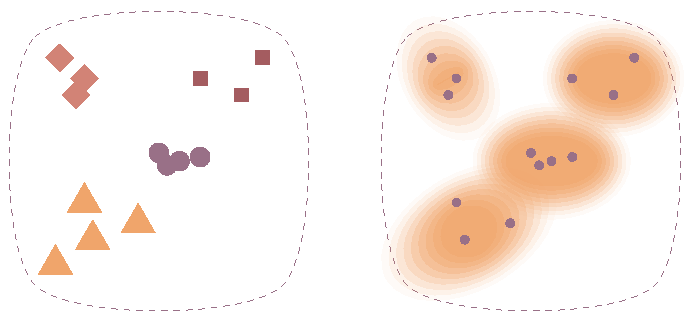
\includegraphics[width=\textwidth*3/4]{chapter1/disc_gen.pdf}
	\caption[Generative modeling]{Discriminative modeling vs Generative modeling. Left: Discriminative modeling, the model aims to assign a target label to each sample. Right: Generative modeling, the model aims to learn the underlying probability distribution of the data.}
	\label{fig:disc_gen}
\end{figure}


We introduce recent approaches such as variational auto-encoders (\ac{VAE}s) \citep{Kingma2014b}, flow methods \citep{Dinh2017, Kingma2018} and the techniques they used to overcome this restriction and train models through maximum likelihood estimation. 



\subsection{Generative modeling with maximum likelihood estimation}

Generative modeling is the task of learning a statistical model of the underlying probability distribution of some observable variable in order to generate samples from that distribution. In other words, it describes how data are generated in terms of a probabilistic model. Indeed,  whereas a classification model tries to find decision boundaries by fitting a parametric model $\pt{Y|X}$ (with parameter $\theta$)  to a conditional probability distribution $\p{Y|X}$ of data $\vx\in\setX$ and label $\vy \in \setY$, a generative model aims to fit $\pt{X}$ to $\p{X}$  the intrinsic marginal distribution of the data and to provide a sampling mechanism based on $\pt{X}$ (\seefigure{fig:disc_gen}).

Learning a discriminative model (\citeq{eq:disc_mle}) and a generative one (\ \citeq{eq:gen_mle}) can be formulated as a maximum log-likelihood estimation
\begin{equation}
		\label{eq:disc_mle}
		\theta^* = \arg\max_\theta \esp{\vx,\vy\sim\p{Y|X}} \log\pt{Y|X}
\end{equation}

\begin{equation}
		\label{eq:gen_mle}
		\theta^* = \arg\max_\theta \esp{\vx\sim\p{X}} \log\pt{X}
	\end{equation}
%
An simple example of generative model are Gaussian Mixture Models (\ac{GMM}) . Given $\vx\in\spaceR^d$, they consist in a sum of $k$ Gaussian distributions $\mathcal{N}(\mu_i, \Sigma_i), 1 \leq i \leq k, \mu_i\in\spaceR^d, \sigma_i\in\spaceR^{d\times d}$  which are all attributed a selection probability $\p{Z}(z=i) = \pi_i$, with $\vz \in \setZ$, so that $\p{X|Z=i} = \mathcal{N}(\mu_i, \Sigma_i)$ . The \ac{GMM} is then formulated as 
%
\begin{equation}
	\pt{X}(\vx) = \sum_{\vz}\p{Z}(\vz)\pt{X|Z}(\vx|\vz)\enspace,
\end{equation}
%
with the log-likelihood 
%
\begin{equation}
	\log\sum_{\vx\sim\p{X}}\pt{X}(\vx)  = \sum_{\vx\sim\p{X}}\log\sum_{i=1}^k \pi_i \mathcal{N}(\vx|\mu_i, \Sigma_i)\enspace.
\end{equation}
%
The Expectation-Maximization (EM) algorithm \citep{Dempster1977} can be used to find the parameters $\theta^*$ maximizing the log-likelihood for such a model. Once the model is trained, sampling a new data is done by picking a component $k$ from the distribution $\p{Z}$ and then drawing a sample from the Gaussian distribution $\p{X|Z=i} = \mathcal{N}(\mu_i^*, \Sigma_i^*)$.

\subsection{Latent variable models}

\begin{figure}
	\centering
	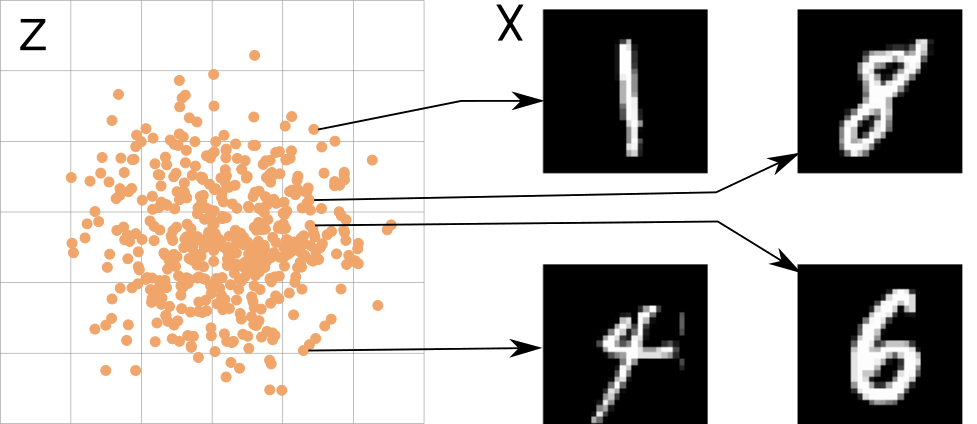
\includegraphics[width=\textwidth]{chapter1/latent_model_full}
	\caption[Latent variable model]{A mapping between a latent space $\setZ$ and the high-dimensional space of an image set $\setX$.}
	\label{fig:latent_space}
\end{figure}


For \ac{GMM}s, sampling a new point consists in, once the components have been selected, sampling a point according to a normal distribution.  This sampling can be done by using reparametrization: instead of directly sampling $\vx \sim \mathcal{N}(\mu_k^*, \Sigma_k^*)$, one can sample a latent variable $\vz \sim \mathcal{N}(0, \mi)$ and compute $\vx = \G(\vz; \mu, \Sigma) = \mu + \Sigma\vz$.  Such a model, that consists in a deterministic function $\G: \spaceZ \rightarrow\spaceX$ between $\spaceZ$ the latent variable space and $\spaceX$ the space of the data, with parameters $\theta$ ($\theta=(\mu,\Sigma)$ in this case) applied to a random latent variable drawn from a fixed distribution $\p{Z}$ is a latent variable model (see Figure \ref{fig:latent_space}).

Since more complex distributions do not necessarily provide a simple sampling mechanism, using a latent variable model allows to outsource the stochastic part of the sampling  process from the learning process and to only learn the deterministic function $\G(\vz; \theta)$. More formally, instead of directly modeling $\p{X}$, a latent variable model learns a deterministic mapping $\pg{X|Z}$. From this mapping, the full generative model can be obtained through marginalization 
%
\begin{equation}
	\pg{X}(\vx) = \int_\setZ \p{Z}(\vz) \pg{X|Z}(\G(\vz;  \theta)) d\vz \enspace .
\end{equation}
%
The marginalization allows for the use of an arbitrary flexible $\G$. However, the actual evaluation of $\pg{X}$ is very likely to be intractable due to the integral over $\setZ$, which prevents the training of such a model as is. While the marginal distribution $\pg{X}$ cannot be explicitly computed for any function $\G$, several solutions exist to overcome this problem. Hereafter, we describe some latent-variable methods to train deep generative models.

\subsubsection{Variational Auto-Encoders}
\label{sub:deep_gen_modeling}

\begin{figure}
	\centering
	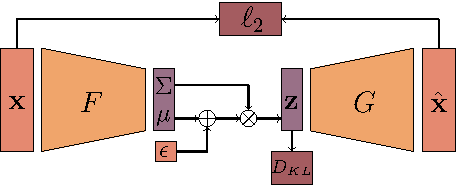
\includegraphics[width=\textwidth*3/4]{chapter1/vae.pdf}	%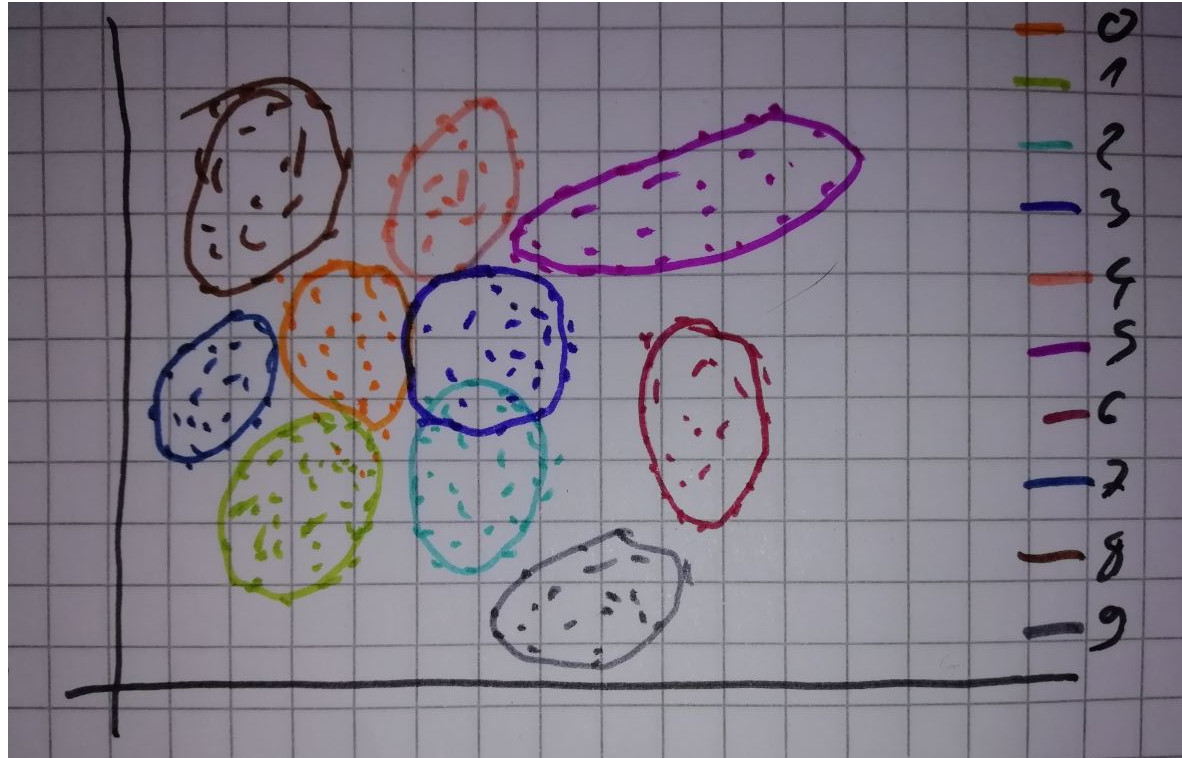
\includegraphics[height=\textheight/5,width=\textwidth*2/5]{chapter1/vae_latent.jpg}
	\caption[Variational auto-encoder]{ Variational auto-encoder framework}
	\label{fig:vae}
\end{figure}

Variational Auto-Encoders (\ac{VAE}) \citep{Kingma2014b}  are deep latent variable models that learn the distribution of the latent model $\pg{X|Z}$ using an auto-encoder approach to train the generative model. In classical auto-encoders, two functions $\F: \setX \rightarrow \setZ$ and $\G: \setZ \rightarrow \setX$ are learned jointly by minimizing
%
\begin{equation}
		L_{AE}	 = \esp{\vx\sim\p{X}} ||\vx - \G(\F(\vx))|| \enspace,
\end{equation}
%
where $||.||$ is usually a $\ell_1$, $\ell_2$ or Frobenius norm, $F$ is an encoding function that maps $\vx$ to a latent representation $\Hat{\vz} = F(\vx)$ and $G$ is a decoding function that maps a latent variable $\vz$ to a sample $\Hat{\vx} = G(\vz)$. However, in the case of generative modeling, $\vz$ needs to be sampled from a random distribution so that generating a new sample $\Hat{\vx}$ can be done by sampling $\vz\sim\p{Z}$ and computing $\Hat{\vx} = \G(\vz)$, with $\p{Z}$  usually chosen to be $\mathcal{N}(0, \mi)$, with $\mi$ the identity matrix. To do so, the \ac{VAE} approach uses the so-called \textit{reparametrization trick}, that consists in having $\F(\vx)$ output the mean and the covariance matrix $(\mu_\vx, \Sigma_\vx)$ of a normal distribution for each sample $\vx$. By first sampling a random vector $\epsilon\in\spaceR^p$ as $\epsilon \sim  \mathcal{N}(0,\mi)$, and using it as a parameter to the model, the random latent code $\vz\sim\p{X|Z}$ can be computed as $\vz = \mu_\vx+\Sigma_\vx\epsilon$. This is equivalent to sampling $\vz \sim \mathcal{N}(\mu_\vx, \Sigma_\vx)$ and is differentiable by considering $\epsilon$ as a parameter. To train the model $\F$, \ac{VAE}s minimize the Kullback-Leibler (\ac{KL}) divergence between the distribution $\mathcal{N}(\mu_\vx, \Sigma_\vx)$ learned by the encoder and the real distribution $\p{Z|X}$, and since $\p{Z}$ is chosen Gaussian, this KL terms can be explicitly computed as
%
\begin{equation}
	\DKL{\mathcal{N}(\mu_\vx, \Sigma_\vx)}{\mathcal{N}(0,I)} = \frac{1}{2}\Big(Tr(\Sigma_\vx) + \mu_\vx^\top\mu_\vx - d - \log(\det\Sigma_\vx)\Big) \enspace,
\end{equation}
%
with $d$ being the dimension of the distribution $\mathcal{N}(0,I)$. By combining the auto-encoder and \ac{KL} terms, we get the objective function of the \ac{VAE} (summed up in Figure \ref{fig:vae}) defined as
%
\begin{equation}
	L_{VAE}(\F, \G) = \esp{\vx \sim \p{X}}\big[ ||\vx - \G(\F(\vx))||^2_2 \big] - \DKL{\mathcal{N}(\mu_\vx, \Sigma_\vx)}{\p{Z}}
\end{equation}
%
Once the model is trained, generating a new sample $\Hat{\vx}$ then consists in sampling a random vector $\vz \sim \mathcal{N}(0, \textbf{1})$ and computing $\Hat{\vx} = \G(\vz)$.

\subsubsection{Normalizing flows}

\begin{figure}
	\centering
	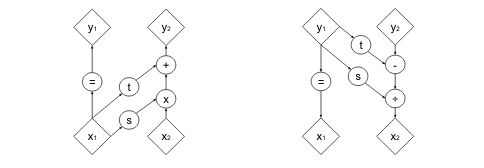
\includegraphics[width=\textwidth]{chapter1/realnvp}
	\caption[RealNVP affine transformations]{The affine transformation used in RealNVP. Left: Forward pass, Right: backward pass. A variable $\vx$ is split in two variables $\vx_1$ and $\vx_2$. The non-linear functions $s(\vx_1)$ and $t(\vx_1)$ are then used to compute the output variables $\vy_1 = \vx_1$ and $\vy_2 =  s(\vx_1) \vx_2 + t(\vx_1)$. Inverting this transformation can then be done by computing $\vx_1 = \vy_1$ and $\vx_2 =  (\vy_2 / s(\vy_1)) - t(\vy_1)$.  Figure by \citet{Dinh2017}}
	\label{fig:realnvp}
\end{figure}

Normalizing flow based techniques are latent variable models that aim to tackle the marginalization problem by using the \textit{change of variable formula}
%
\begin{equation}
	\pg{X} = \p{Z} \Big|\det\Big(\frac{\partial\G(\vz)}{\partial{\vz^T}}\Big)\Big|^{-1}  = \p{\G^{-1}_X} \Big|\det\Big(\frac{\partial\G^{-1}(\vx)}{\partial{\vx^T}}\Big)\Big|  \enspace ,
	\label{eq:change_variable_formula}
\end{equation}
%
with $\vz \sim \p{Z}$ a latent variable. This formulation has notable advantages such as explicitly allowing the computation of the exact inference, that is to compute $\vz$ such that $\vx = G(\vz)$ for any given sample $\vx$. However, the model has to enforce some tough constraints: the input and output dimensions must be the same; $\G$ must be invertible; and the computation of the determinant of the Jacobian needs to be efficient and differentiable. These constraints can be enforced through strong restrictions on the architecture of the model. By limiting the transformations to a set of invertible transformations with a tractable Jacobian determinant, the model remains invertible and the determinant of its Jacobian can be computed efficiently.

\textbf{Real-valued non-volume preserving (RealNVP)} normalizing flows \citep{Dinh2017} uses affine coupling transforms, which converts a set of variable by adding and scaling it by a non-linear transformation, usually computed with deep neural networks (see Figure \ref{fig:realnvp}). These transformations can be inverted by substracting and downscaling by the same transformed variables. Their Jacobians are triangular, therefore computing the determinants can be done efficiently by computing the product of their diagonal terms.  \textbf{\textit{Glow}} \citep{Kingma2018} extended this set of transformations to $1\times1$ invertible convolutions as well as a variant of batch normalization \citep{Ioffe2015} that allows for more expressiveness in the model.

%$\vx$ into $\vy$ by partitioning it into $(\vx_1, \vx_2)$ and computing $\vy_1 = \vx_1; \vy_2 = \exp(s_\theta(\vx_1)) \odot \vx_2 + m_\theta(\vx_1)$, where $s_\theta$ and $m_\theta$ are arbitrary scaling and translation parametric functions. These transformations can be inverted as $\vx_1 = \vy_1; \vx_2 = \exp(-s_\theta(\vy_1)) \odot (\vx_2 - m_\theta(\vx_1))$ 


\section{Generative Adversarial Networks}

As for the latent-variable generative models, Generative Adversarial Networks (\ac{GANs}) \citep{Goodfellow2014} aim to learn a mapping between samples  from the latent distribution (usually normal or uniform) and samples from the data distribution. However, instead of directly relying on the likelihood and trying to estimate the distribution through marginalization, it aims to minimize the distance between the modeled distribution and the real data distribution.  Therefore, \ac{GANs} are sometimes qualified as \textit{likelihood-free} generative models.

We denote the generative model as a mapping $\pg{X|Z}$, where $\G: \spaceZ \rightarrow \spaceX$ is a deterministic function, that maps samples $\vz \sim \p{Z}$ from the latent distribution $\p{Z}$ and samples $\vx\sim\p{X}$ from the the real data distribution. We define the modeled distribution as $\pg{X} = \pg{X|Z}\sharp\p{Z}$\footnote{$\sharp$ is the push-forward operator that transfers a measure (in this case, a probability distribution) from one measurable space to another using a function. Here, $\pg{X|Z}\sharp\p{Z}$ represents the distribution obtained by "pushing" $\p{Z}$ through the function $G$.}.

In this section, we introduce the formulation of adversarial learning as an approximation of a divergence. Leveraging this formulation, we present the Generative Adversarial Networks framework as a pair of models, the generator model and a discriminator model, which is a binary classifier that aim to distinguish real and generated samples. Training these two models as a min-max problem, using alternate gradient descent, approximates the minimization of the Kullback-Leibler divergence between the real data distribution and the distribution of generated samples. We discuss some limitations of this model, most notably stability issues implied by alternate gradient descent, and the lack of statistical diversity.

\subsection{Generative modeling through divergence approximation}

A divergence $\Div{\p{X}}{\q{X}}$ between two distributions $\p{X}$ and $\q{X}$ is a weak form of distance between these distributions (\seefigure{fig:divergence}), thus minimizing such a divergence allows for a parametric distribution $\pt{X}$ that fits a target distribution $\p{X}$. Whenever the divergence is both tractable and differentiable w.r.t the parameters $\theta$, stochastic gradient descent can be used to estimate $\theta$, thus allowing for the training of a generative model.

\begin{figure}
	\centering
	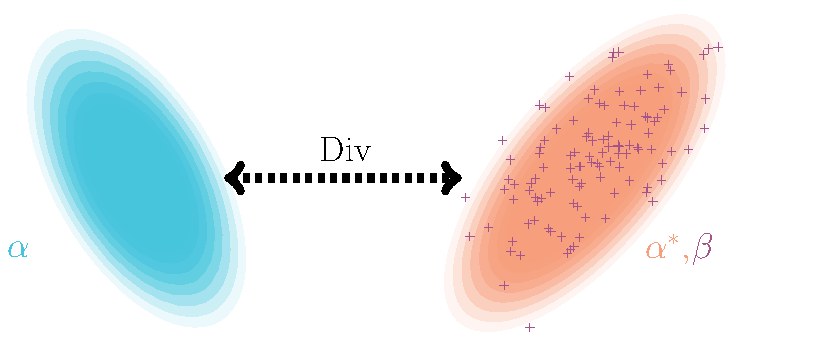
\includegraphics[width=\textwidth*3/4]{chapter1/div.pdf}\hspace{-2cm}
	\caption[Illustration of a divergence]{A divergence $\Div{\alpha_\theta}{\beta}$ can capture the distance between a parametric density model $\alpha_\theta$ and the distribution $\beta$ from which a set of samples are observed. Density fitting can then be formulated as  finding $\theta^* = \arg\min_\theta \Div{\alpha_\theta}{\beta}$, such that $\alpha_{\theta^*}$ is the best fit model.}
	\label{fig:divergence}
\end{figure}

However in practice, such divergences are usually intractable in the case of generic distributions. Hence \ac{GAN}s aim to estimate the divergence by relying on another learnable function that will act as a surrogate to the divergence, the discriminator model $\D$. This discriminator is trained as a binary classifier that predicts the probability of a sample $\vx$ to be issued from the real distribution $\p{X}$ or generated from $\pg{\vx}$ using binary cross-entropy (see Figure \ref{fig:gan}) as
%
\begin{equation}
	\label{eq:disc_cost}
	L_\D(\D, \G) =  \esp{\vx\sim \p{X}} [\log \D(\vx)] +  \esp{\Hat{\vx}\sim\pg{\vx}} [1 - \log \D(\Hat{\vx})] \enspace .
\end{equation}
%
The intuition behind this model is that once the discriminator is trained, maximizing its error on generated samples $\Hat{\vx}\sim\pg{X}$ w.r.t $\G$ will push $\pg{X}$ towards $\p{X}$.

\begin{figure}
	\centering
	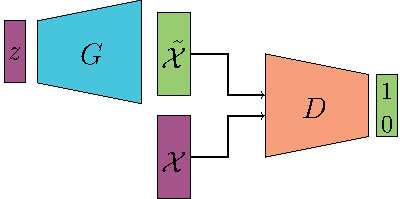
\includegraphics[width=\textwidth*2/3]{chapter1/gan.pdf}
	\caption{Generative Adversarial Network framework}
	\label{fig:gan}
\end{figure}

As the optimum of $f(x) = a\log(x) + b\log(1-x)$ is $\frac{a}{a+b}$, the discriminator that maximizes $L_\D(\D, \G)$ for a fixed $\G$ is given by

\begin{equation}
\label{eq:optimal_D}
\D^*_\G(\vx) = \frac{\p{X}(\vx)}{\p{X}(\vx) + \pg{X}(\vx)} \enspace.
\end{equation}

By plugging back Equation \ref{eq:optimal_D} into $L_D(\D, \G)$ (Equation \ref{eq:disc_cost}), we get
\begin{equation}
		\max_\D L_\D(\D,\G) =  \esp{\vx\sim \p{X}} \Big[\log \frac{\p{X}(\vx)}{\p{X}(\vx) + \pg{X}(\vx)}\Big] +   \esp{\vx\sim \pg{X}} \Big[1 - \log  \frac{\p{\vx}(\vx)}{\p{X}(\vx) + \pg{X}(\vx)}\Big] \nonumber \enspace.
\end{equation}

As said previously, the objective of the generator model $\G$ will be to maximize the error of the discriminator $\D$. Thus, we can formulate the objective function $L_\G(\G)$ related to $\G$ as $L_\G(\G) = \max_\D L_\D(\D,\G)$. Up to additive and multiplicative constants, $L_\G(\G)$ can be reformulated \citep{Goodfellow2014} as

\begin{equation}
		\label{eq:gen_cost}
		L_\G(\G) = \DKL{\p{X}}{\frac{\p{X}+\pg{X}}{2}} + \DKL{\pg{X}}{\frac{\p{X}+\pg{X}}{2} } = 2\cdot\JSD{\p{X}}{\pg{X}} \enspace.
\end{equation}

Assume the discriminator is trained to convergence. Minimizing $L_\G( \G) $ is therefore equivalent to minimizing the Jensen-Shannon (\ac{JS}) divergence between $\p{X}$ and $\pg{X}$.  This training process is summarized as the mini-max problem
%
\begin{equation}
\label{eq:GAN_problem}
\arg\min_\G\min_G\lgan = \arg\min_\G\max_\D \esp{\vx\sim \p{X}} [\log \D(\vx)] +  \esp{\vz\sim\p{Z}} [1 - \log \D(\G(\vz))] \enspace.
\end{equation}
%
From Equation \ref{eq:gen_cost},  we find that the mini-max game has, assuming infinite capacity for both $\G$ and $\D$, a global optimum for $\p{X} = \pg{X}$. The \ac{GAN} training algorithm then consists in alternatively updating the discriminator and the generator via gradient ascent/descent respectively. A summary of this process is presented in \citealg{alg:GAN_train}. 

\begin{algorithm}[!ht]
	\caption{The \ac{GAN} training algorithm}
	\label{alg:GAN_train}
	\begin{algorithmic}[H]
		\REQUIRE{$\trainsetX$ the real dataset, $\G$ the generator and $\D$ the discriminator models}
		\REPEAT
		\STATE sample a mini-batch $\lbrace \vx_i \rbrace_{i=1}^m$ from $\trainsetX$\;
		\STATE sample a mini-batch $\lbrace \vz_i \rbrace_{i=1}^m$ from distribution $\p{Z}$\;
		\STATE update $\D$ by stochastic gradient ascent of
		\STATE \ \ \ \ $\sum_{i=1}^{m}\log(\D(\vx_i)) + \log(1-\D(\G(\vz_i)))$
		\STATE sample a mini-batch $\lbrace \vz_j \rbrace_{j=1}^n$ from distribution $\p{Z}$\;
		\STATE update $\G$ by stochastic gradient descent of
		\STATE \ \ \ \ $\sum_{j=1}^n \log(1-\D(\G(\vz_j)))$\;
		\UNTIL a stopping condition is met
		
	\end{algorithmic}
\end{algorithm}

\subsection{Conditional modeling with generative adversarial networks}
\label{subs:CGAN}

While classical generative models such as \ac{GAN}s try to unconditionally approximate the real-data distribution $\p{X}$, a conditional generative model aims to match the conditional distribution $\p{X|Y}$ related to $\p{X,Y}$ the joint distribution that constitutes the data, where $y \in \setY$ is a label of any kind.

\begin{figure}
	\centering
	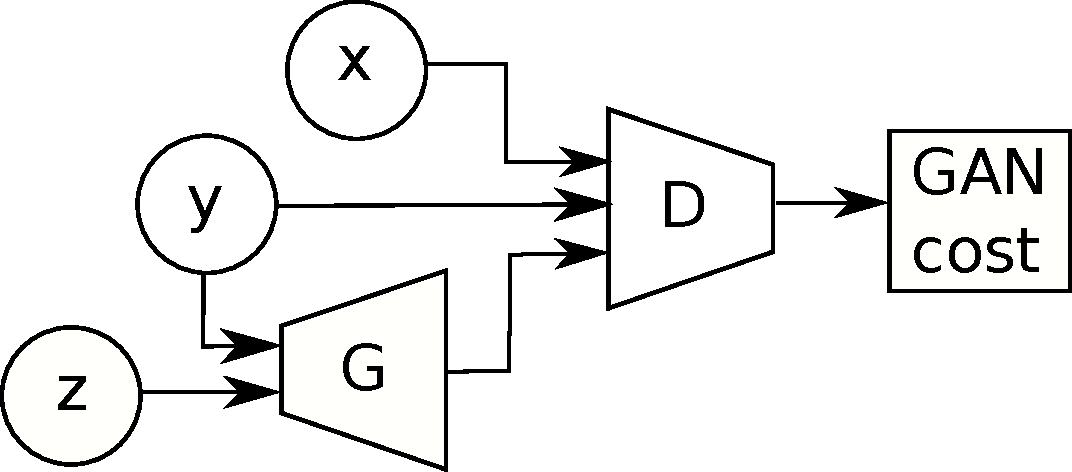
\includegraphics[width=\textwidth*3/5]{chapter1/cgan}
	\caption[Conditional GAN approach]{Conditional Generative Adversarial Networks}
	\label{fig:cgan}
\end{figure}

Several extensions to the \ac{GAN} framework allow for conditional modeling: \textbf{Conditional \ac{GAN}s (\ac{CGAN}s)} \citep{Goodfellow2014, Mirza2014}, simply adds the label $y$ as an input for both the discriminator and the generator (see Figure \ref{fig:cgan}). It results the optimization problem
%
\begin{equation}
	\label{eq:CGAN_problem}
	\arg\min_\G\max_\D \lcgan = 	\arg\min_\G\max_\D \esp{\vx,\vy\sim \p{X,Y}} [\log \D(\vx, \vy)] +  \esp{\vy\sim \p{Y} \\ \vz\sim\p{Z}} [1 - \log \D(\G(\vy, \vz), y)]
\end{equation}
%
Other approaches such as \textbf{Auxillary Classifier GAN (ACGAN)} \citep{Odena2016}  try to learn the conditional distribution by adding an explicit loss term to the optimization problem. ACGAN aims to learn a conditional generative model with discrete labels by adding another output, with dimension $n$ equal to the number of labels, to the discriminator that acts as a classifier $C$ sharing its weights with the discriminator (see Figure \ref{fig:acgan}). The model is then trained by having both the generator and the discriminator minimize the categorical cross-entropy  between the real and predicted labels.

\begin{figure}
	\centering
	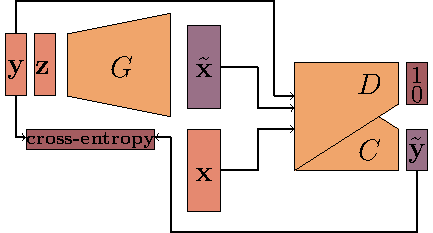
\includegraphics[width=\textwidth*3/5]{chapter1/acgan}
	\caption[Auxiliary Classifier GAN approach]{Auxiliary Classifier Generative Adversarial Networks approach.}
	\label{fig:acgan}
\end{figure}


\begin{align}
	\label{eq:ACGAN_problem}
	L_{ACGAN_{\D}}(\D, \G) &= \lgan(\D, \G) + \esp{(\vx, \vy) \sim\p{X,Y}} \Big[ -\sum_{i=1}^{n} \vy_i C(\vx)_i \Big]\\
	L_{ACGAN_{\G}}(\D, \G) &= \lgan(\D, \G) - \esp{\vy\sim\p{Y}\\\vz\sim\p{Z}} \Big[ -\sum_{i=1}^{n} \vy_i C(\G(\vz))_i \Big]
\end{align}

\begin{figure}
\centering
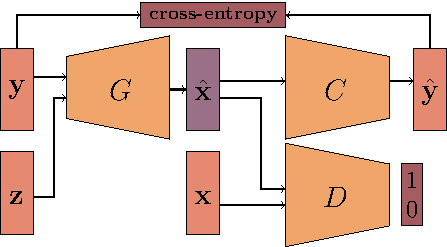
\includegraphics[width=\textwidth*3/5]{chapter1/triplegan}
\caption[Triple GAN approach]{Triple Generative Adversarial Network approach.}
\label{fig:triplegan}
\end{figure}

\textbf{TripleGAN} \citep{Li2017} considers a classifier $C$, disjoint from $D$, which can be pre-trained  or learned jointly to the GAN models. This classifier is then used to train the generator to generate images whose label $\Hat{\vy} = C(\G(\vy, \vz)), \vy\sim\p{Y}, \vz\sim\p{Z}$ actually corresponds to the original label $\vy$ (see Figure \ref{fig:triplegan}). This is done by adding a classification loss to the GAN objective function, as

\begin{equation}
	L_{TripleGAN}(\D, \G, C) = L_{GAN} (\D, \G) + \esp{\vy\sim\p{Y}\\\vz\sim\p{Z}} \Big[-\sum_{i=1}^{n} \vy_i \log C(\G(\vy, \vz)) \Big] \enspace.
\end{equation}

\subsection{Domain-transfer approaches using generative adversarial networks}
\label{subs:domain_transfer}

Domain-transfer is the task of learning a mapping $\G_{YX}:\spaceX\rightarrow\spaceY$ such that the generated samples $\Hat{\vx}$ are issued from the distribution $\p{X}$ while maintaining some semantic information. This can be, for example, changing the color palette of an image, or transforming a photo of an object into a painting of the same object (see Figure \ref{fig:cyclegan_samples}).

Several approaches exist for domain-transfer \citep{Isola2016, Taigman2017} that require paired samples $\{(\vx_1, \vy_1),  ..., (\vx_s, \vy_s)\},  \vx_i \in \spaceX, \vy_i \in \spaceY$ from both domains. \ac{CGAN}s already learn to model the conditional distribution $\p{X|Y}$, and adding a way to enforce the consistency of the semantic information enables domain-transfer.

\textbf{Pix2Pix} \citep{Isola2016} implemented this approach  explicitly by using paired samples $(\vx, \vy) \sim \p{X,Y}$ and by forcing the generator to minimize a reconstruction term (in this case, the authors choose the $\Lone$ norm) between $\vx$ and $\G(\vy,\vz)$ (see Figure \ref{fig:pix2pix}) as
%
\begin{equation}
	\arg\min_{\G_{YX}}\max_\D L_{p2p} =  \arg\min_{\G_{YX}}\max_\D \lcgan(\D, \G) +\lambda\esp{(\vx, \vy)\sim\p{X,Y}\\\vz\sim\p{Z}} ||\vx - \G_{YX}(\vy, \vz)||_1 \enspace .
\end{equation}


\begin{figure}
	\centering
	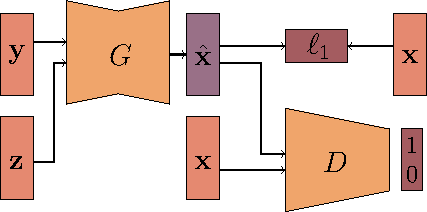
\includegraphics[width=\textwidth*3/5]{chapter1/pix2pix}
	\caption[Pix2Pix approach]{Pix2Pix domain-transfer approach}
	\label{fig:pix2pix}
\end{figure}

\begin{figure}
	\centering
	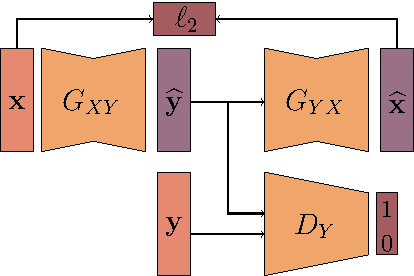
\includegraphics[width=\textwidth*3/5]{chapter1/cyclegan}
	\caption[CycleGAN approach]{The CycleGAN approach. Half of the training setup is illustrated, the other half consisting in the same setup but with inverted $\vx$ and $\vy$}
	\label{fig:cyclegan}
\end{figure}

\begin{figure}
	\centering
	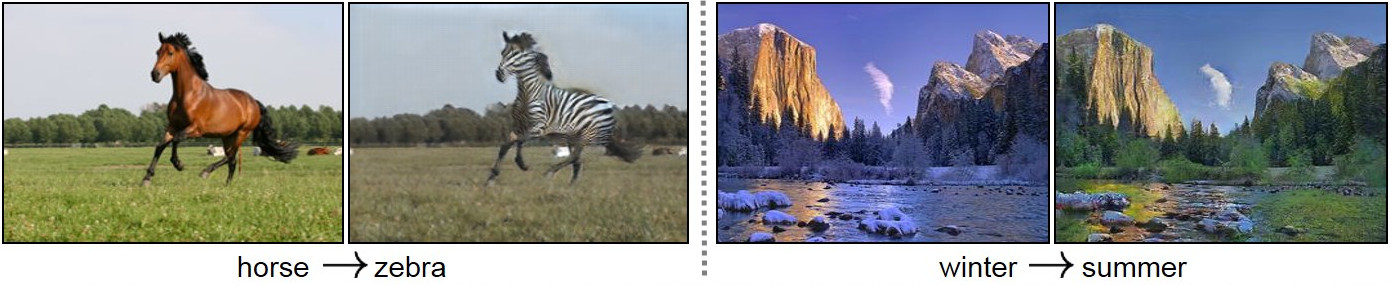
\includegraphics[width=\textwidth]{chapter1/cyclegan_samples}
	\caption[Examples of domain-transfer with CycleGAN]{Examples of domain-transfer with CycleGAN \citep{Zhu2017a}. For this kind of images,  paired data can be hard to acquire.}
	\label{fig:cyclegan_samples}
\end{figure}

\noindent However, these approaches rely on paired data which can be very hard to obtain, especially in the case of natural images. \citet{Zhu2017a} present an example of this issue with a domain-adaptation task, in which a model turns images of horses into zebras. In such a case, it is very hard to get paired images of identical zebras and horses (see Figure \ref{fig:cyclegan_samples}). A solution to this problem of paired data was proposed in the form of \textbf{cyclic consistency} \citep{Zhu2017, Kim2017, Liu2018a, Yi2017}. Instead of training a single model $\G_{XY}$ with a reconstruction loss between $\vx$ and $\G(\vy)$, the cycle-consistent approaches train two domain-transfer models simultaneously: $\Gyx$ and $\Gxy$ that push-forward $\p{Y}$ onto $\p{X}$ and $\p{Y}$ onto $\p{X}$, respectively (\seefigure{fig:cyclegan}). This allows to compute the reconstruction errors  $||\vx - \Gyx(\Gxy(\vx))||_1$ and $||\vy - \Gxy(\Gyx(\vy))||_1$, which ensure that the content of the image is preserved through the mappings.  Note that these reconstruction errors do not require paired data $(\vx,\vy)$. 

The training of the two models in done an adversarial setup, with two discriminators $\Dx$ and $\Dy$, and is wrapped up in the \textbf{\ac{CycleGAN}} approach \citep{Zhu2017a} as
%
\begin{align}
	\label{eq:cyclegan}
	\min_{\Gxy, \Gyx}\max_{\Dx, \Dy} & \enspace \lcycgan  (\G_{XY}, \G_{YX}, \D_X, \D_Y) = \nonumber \\ 
	\min_{\Gxy, \Gyx}\max_{\Dx, \Dy}  &\enspace \lgan(\G_{YX}, \D_{X}) +\lgan(\G_{XY}, D_{Y}) \nonumber \\
	& +\lambda \Big[ \esp{\vx\sim\p{X}} ||\vx - \Gyx(\Gxy(\vx))||_1 + \esp{\vy\sim\p{Y}} ||\vy - \Gxy(\Gyx(\vy))||_1 \Big] \enspace .
\end{align}
%
The \ac{CycleGAN} training process then consists in alternatively updating the two discriminators and the two generators via gradient ascent/descent (\citealg{alg:cyclegan_train}). Note that, as opposed to the previous approaches, \ac{CycleGAN} does not use random vectors $\vz\in\p{Z}$ to generate images. The stochastic part of the generation process is instead contained in the initial image $\vy\sim\p{Y}$

\ac{CycleGAN}, as well as similar methods relying on cycle-consistency such as \textbf{DualGAN} \citep{Yi2017} or \textbf{DiscoGAN} \citep{Kim2017}, have been used in several domains. Among them are medical imaging \citep{Chen2019}, training models with synthetic images obtained with a simulator, for example for robot grasping \citep{Bousmalis2018}), for image segmentation \citep{Perone2019} or for converting near-infrared images to color images \citet{Sun2019}. These approaches shows that even conversion between different image modalities can be done with cycle-consistent generative models.

\begin{algorithm}
	\begin{algorithmic}[]
		\REQUIRE{$\trainsetX$ and $\trainsetY$ two unpaired datasets, $\Gxy$ and $\Gyx$ the mapping networks, $\Dx$ and $\Dy$ the discrimination models, $m$ the mini-batch size, $\lambda$ a hyperparameter}
		\REPEAT
		\STATE sample a mini-batch $\lbrace \vx_i \rbrace_{i=1}^m$ from $\trainsetX$\;
		\STATE sample a mini-batch $\lbrace \vy_i \rbrace_{i=1}^m$ from $\trainsetY$\;
		\STATE update $\Dx$ by stochastic gradient ascent of $ \sum_{i=1}^{m}\big( \lgan(\G_{YX}, \D_{X})\big)$\;
		\STATE update $\Dy$ by stochastic gradient ascent of $ \sum_{i=1}^{m}\big(\lgan(\G_{XY}, D_{Y})\big)$\;
		\STATE update $\Gxy$ by stochastic gradient descent of
		\STATE \ \ \ \ $ \sum_{i=1}^m \big(\lgan(\G_{YX}, \D_{X})\big)  + \lambda \big(||\vx_i - \Gyx(\Gxy(\vx_i))||_1 +||\vy_i -\Gxy(\Gyx(\vy_i))||_1\big)$\;
		\STATE update $\Gyx$ by stochastic gradient descent of
		\STATE \ \ \ \ $ \sum_{i=1}^m \big(\lgan(\G_{XY}, D_{Y})\big)+ \lambda\big (||\vx_i - \Gyx(\Gxy(\vx_i))||_1 + ||\vy_i - \Gxy(\Gyx(\vy_i))||_1\big)$\;
		\UNTIL a stopping condition is met
	\end{algorithmic}
	\caption{CycleGAN training algorithm}
	\label{alg:cyclegan_train}
\end{algorithm}

\subsection{Limitations}
\label{sub:limitations}

GANs have shown strong advantages over the classical generative modeling methods, such as generating sharper samples than \ac{VAE}s and normalizing flows \citep{Danihelka2017}. They however bear limitations, namely the instability of the training procedure and the lack of diversity in the generated samples (\textit{mode-collapse}).

\subsubsection{Instability}

Training \ac{GAN}s consist in solving a minimax problem. While the alternate gradient descent algorithm is a common method for solving such a problem, the alternating updates can cause significant instabilities during the training process. This can result in oscillating values of the \ac{GAN} objective function which prevents the optimization from converging \citep{Mescheder2018} and makes it difficult to set a stopping criterion.

\begin{figure}
	\centering
	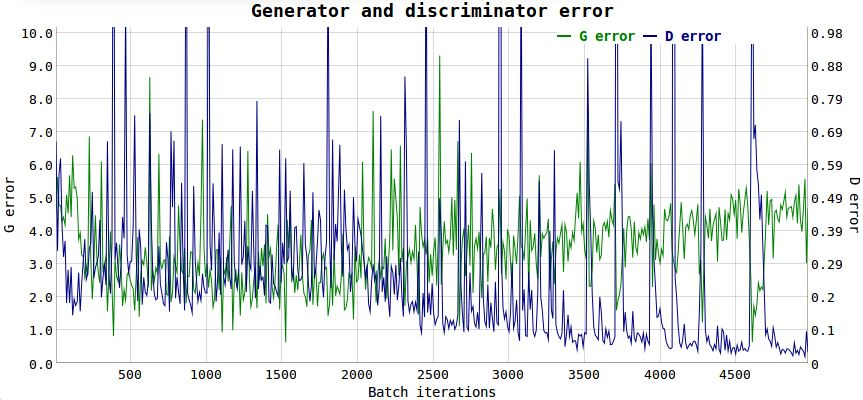
\includegraphics[width=\textwidth]{chapter1/crazy_loss_function}
	\caption[Instability in the training process]{Examples real losses during the training of a \ac{GAN}.}
	\label{fig:crazy_loss_function}
\end{figure}

The instability of the \ac{GAN} training has first been conjectured to be caused by the bad quality of the gradients obtained when $\G$ generates bad samples, which makes $\D$ strongly reject these samples and therefore saturating the loss. A proposed solution \citep{Goodfellow2014} was to slightly change the generator's loss function from $\log(1-\D(\G(\vz)))$ to 
%
\begin{equation}
	\label{eq:nsgan}
	\L_G(D, G) = -\esp{\vz\sim\p{Z}}\log(\D(\G(\vz)))
\end{equation}, which helps considerably in avoiding failures of the training process \citep{Radford2015}.
%
 While this new loss function converges to the same minimum as the original loss term, minimizing it no longer correspond to minimizing a \ac{JS} divergence but the non-symmetric reverse \ac{KL} divergence, minus a \ac{JS} term \citep{Arjovsky2017a}. More formally, 

\begin{equation}
	\esp{\vz\sim\p{Z}}\Big[\nabla_\G\log\D^*(\G(\vz))\Big] = \nabla_\G\Big[\DKL{\pg{X}}{\p{X}} - 2\JSD{\pg{X}}{\p{X}}\Big] \enspace .
\end{equation}

\begin{figure}
	\centering
	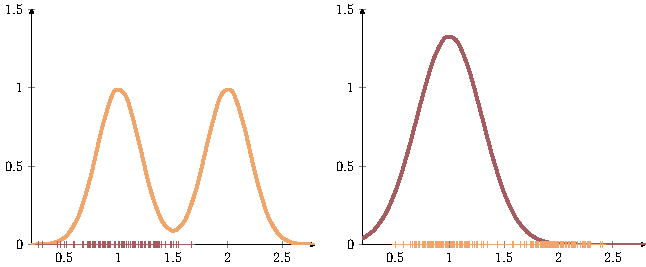
\includegraphics[width=\textwidth]{chapter1/kl_rkl.pdf}
	\caption[\ac{KL} and reverse \ac{KL} divergence]{Reverse \ac{KL} (left) and \ac{KL} (right) divergence between the true orange distribution and the mode-collapsed purple distribution. When computing these distances, the reverse \ac{KL} is lower, even if a missing mode is clearly visible.}
	\label{fig:kl_rkl}
\end{figure}

\noindent However, albeit an empirical reduction of the instability, this new loss has been proved to not solve the instability problem \citep{Arjovsky2017a}. One hypothesis for this issue is the degenerate behavior of the \ac{JS} and \ac{KL} divergences when the real distribution and the learned one does not share the same support. Several tricks can be applied to the training process in order to avoid this pitfall \citep{Salimans2016, Sonderby2017, Heusel2017}, such as adding noise on the discriminator input or using separate optimizers for the generator and the discriminator. Although more recent approaches  (more thoroughly detailed in section \ref{sec:improvements}), seem to help alleviate this issue, instability can still be observed in approaches that make full use of them \citep{Brock2018}. Even though several techniques aimed to solve this issue \citep{Arjovsky2017, Nowozin2016, Li2017a}, to our knowledge at the time of writing this thesis, there are neither clear consensus on the theoretical causes of this instability nor robust efficient solutions.


\subsubsection{Mode collapse}
\label{subs:mode_collapse}

Although the aforementioned change of loss from $\log(1-\D(\G(\vz)))$ to $-\log(\D(\G(\vz)))$ can help solving the instability issues, using the reverse \ac{KL} divergence is conjectured to be one reason of the loss of statistical diversity. Reasons of the lack of diversity are twofold: the \textit{mode collapse} problem that causes different $\vz_1, \vz_2$ to be mapped to samples $\G(\vz_1)$ and $\G(\vz_2)$ that are very close;  and  \textit{mode dropping} which leads to missing modes in the generated samples, as only a localized support of the target distribution can actually be mapped to. Indeed, the reverse \ac{KL} divergence does not penalize "missing" parts of the learned distribution $\pg{\vx}$, which correspond top some points in the support of $\p{X}$ that have zero (or near-zero) probability on $\pg{X}$ (\seefigure{fig:kl_rkl}).

Another conjectured cause is raised by the alternate gradient descent. Indeed, this algorithm does not behave in the same way when formulating the problem as a minimax problem $\G^* = \min_\G\max_\D \lgan$ or maximin problem $\G^* = \max_\D\min_\G \lgan$. Most notably, using alternate gradient descent to solve the maximin problem can push the generator towards mapping every $\vz$ to the single most probable $\vx$, evaluated  by the generator \citep{Goodfellow2016}.

As for the instability problem, there is, to our knowledge, no clear consensus on the origin mode collapse. However, a trade-off seems to emerge: using the original \ac{GAN} creates instability which leads to a drop of visual quality, and using the non-saturating variant that stabilizes the training creates a lack of diversity. This extends to more recent approaches in which higher visual quality induces a loss of diversity \citep{Brock2018}.

In the most extreme cases, this loss of diversity can result in a complete collapsing of the sampling mechanism, making it impossible to draw diverse samples. In that case, the generated images $\Hat{\vx} = \G(\vz)$ can be considered independent from $\vz$. This loss of diversity, however, is not as much of an issue for conditional tasks that consists in mapping an input to one of many acceptable outputs, the most notable of these tasks being domain-transfer (see Section \ref{subs:domain_transfer}). 

\section{Improvements to Generative Adversarial Networks}
\label{sec:improvements}

Recently, Generative Adversarial Networks have made progress towards generating realistic high definition images \citep{Brock2018, Karras2020, Wang2018b} (see Figure \ref{fig:biggan_samples}). These notable successes leverage an overwhelming amount of incremental enhancements and variations of the original GAN \citep{Hindupur2017}. In this section, a summary of some GAN variants is proposed. We consider two objectives: enhancing the visual quality of the generated samples and ensuring some diversity among the generated samples. We discuss three categories of approaches for this: changing the optimized divergences through alternative loss functions; regularization, normalization and auxiliary tasks and improvements to the training process; and the architecture of the neural networks.


\begin{figure}
	\centering
	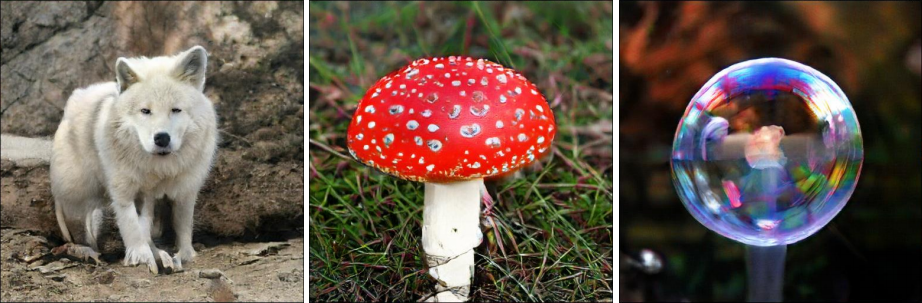
\includegraphics[width=\textwidth]{chapter1/biggan_samples}
	\caption[Samples generated with the BigGAN approach]{Samples generated with the BigGAN approach \citep{Brock2018}. By combining several recent techniques for improving GANs with very large models and datasets, GANs can generate nearly photo-realistic images.}
	\label{fig:biggan_samples}
\end{figure}

\subsection{Changing the divergence}
\label{sec:divergences}

As mentioned in \citesub{sub:limitations}, the original GAN loss (see Equation \ref{eq:GAN_problem}) as well as its non-saturating variation (Equation \ref{eq:nsgan}) show strong limitations, the former causes instability and the latter causes a loss in diversity. As potential solutions, several new loss terms are envisioned.

An alternative to the objective function to the Jensen-Shannon and the reverse Kullback-Leibler divergences is the least-squares loss, which leads to the following discriminator error
%
\begin{equation}
	\loss{LSGAN}(\D, \G) = \esp{\vx\sim\p{X}} \Big[ (1-\D(\vx))^2\Big] + \esp{\vz\sim\p{Z}} \Big[ (\D(\G(\vz)))^2\Big] \enspace .
\end{equation}
%
Such a loss term was considered by \citet{Mao2017} for their \textbf{Least-Squares GAN(\ac{LSGAN})}. While this loss function follow the same idea as in the original GAN method, \ac{LSGAN} actually optimizes Pearson's $\chi^2$ divergence. Empirically, \ac{LSGAN}s show more stability as well as a higher visual quality of the generated samples than the original GAN approach. The reason potentially resides in a better quality of the gradients.

Although showing notable differences in their behavior when optimized, both the Jensen-Shannon, reverse Kullback-Leibler and Pearson $\chi^2$ divergences are part of \textbf{the $f$-divergence family} \citep{Liese2006} defined as 

\begin{equation}
	D_f(\p{X} || \q{X})  =\esp{\vx\sim\q{X}}f\Big(\frac{\p{X}(\vx)}{\q{X}(\vx)}\Big)  \enspace ,
\end{equation}

where $f: \mathbb{R}^+\rightarrow \mathbb{R}$  is a convex, lower-semi-continuous function satisfying $f(1) = 0$. By carefully choosing $f$, we can recover the \ac{KL} ($f(u) =  u\log u$), reverse \ac{KL} ($f(u) =  -\log u$), \ac{JS} ($f(u) =  -(u+1)\log (\frac{u+1}{2} + u\log u)$) and Pearson's $\chi^2$ ($f(u) = (u-1)^2$) divergences. \citet{Nowozin2016} proposed a generalized approach for these divergences as well as several new GAN formulations based on divergences such as the Squared Hellinger distance ($f(u) = (\sqrt{u}-1)^2$) or the Total Variation ($f(u) = \frac{1}{2}|u-1|$). The \textbf{hinge loss} variant for GANs \citep{Lim2017}, which redefines the loss of the discriminator as
%
\begin{equation}
		\loss{{hinge_D}}(\D, \G) = - \esp{\vx \sim \p{X}} \Big[\min(0, \D(\vx) - 1)\Big] - \esp{\vz\sim\p{Z}} \Big[\min(0, -\D(\G(\vz))-1)\Big] \enspace,
\end{equation}
%
can also be expressed as the Reverse Kullback-Leibler divergence \citep{Miyato2018}.

While the $f$-divergences have been the seminal approach to GANs, they can exhibit strong issues. \citet{Arjovsky2017} have shown that these divergences can have degenerate behaviors, most notably when the distributions $\p{X}$ and $\pg{X}$ have no shared support, causing the divergence to be non-continuous and non-differentiable. As a solution to this issue \citet{Arjovsky2017} proposed the \textbf{Wasserstein GAN (\ac{WGAN})} by replacing the Jensen-Shannon divergence by the Wasserstein-1 (or Earth-Mover) distance which stems from optimal transport theory \citep{Peyre2020}.  The Wasserstein distance, albeit having many different formulations, can be expressed in its dual form using the Kantorovich-Rubinstein duality \citep{Kantorovich1982} as
%
\begin{equation}
		W(p||q) = \sup_{f \in \mathcal{F}} \Big[ \esp{\vx\sim\p{X}} f(\vx) - \esp{\vx\sim\q{X}} f(\vx) \Big] \enspace ,
\end{equation}
%
where $\mathcal{F} = \{f:||f||_L\leq1\}$ is the set of 1-Lipschitz functions, $\|.\|_L$ being the Lipschitz norm. By using a parameterized family of functions $D$ (in our case, a neural network), we can formulate the Wasserstein GAN problem as

\begin{equation}
\loss{WGAN}(\D, \G) = \min_G\max_{D\in\mathcal{F}} \Big[ \esp{\vx\sim\p{X}} D(\vx) - \esp{\vz\sim\p{Z}} D(G(\vz)) \Big] \enspace .
\end{equation}


\begin{table}
	\centering
	\begin{tabular}{|c c|}
		\hline
		Approach & Divergence \\
		\hline 
		\hline 
		\multicolumn{2}{|c|}{$f$-divergences} \\
		\hline
		GAN \citep{Goodfellow2014}& Jensen-Shannon \\
		NS-GAN \citep{Goodfellow2014} & Reverse KL - 2$\cdot$Jensen-Shannon\\
		LSGAN \citep{Mao2017}& Pearson $\chi^2$ \\
		EBGAN* \citep{Zhao2017} & Total variation \\
		Geometric GAN \citep{Lim2017} & Reverse Kullback-Leibler \\
		$f$-GAN \citep{Nowozin2016} & Various $f$-divergences\\
		\hline 
		\hline 
		\multicolumn{2}{|c|}{Integral Probability Metrics (\ac{IPM}s)}\\
		\hline
		EBGAN* \citep{Zhao2017} & Total variation \\
		WGAN \citep{Arjovsky2017}& Wasserstein distance \\
		Cramér GAN \citep{Bellemare2017}& Energy Distance (Unbiased WGAN) \\
		MMDGAN \citep{Li2017a}& Maximum Mean Discrepancy \\				
		Fisher GAN\citep{Mroueh2017}& Fisher IPM \\
		\hline
	\end{tabular}
	\label{table:divergences}
	\caption[Summary of common $f$-divergences and \ac{IPM} used to train GANs]{A summary of common $f$-divergences and \ac{IPM} used to train GANs. Note than the Total Variation can be formulated as both.}
\end{table}


This formulation, however, requires the discriminator to be 1-Lipschitz. This property is enforced done by clipping the weights $\mw$ of the discriminator so that each weight $w_{i,j}$ is in a fixed interval $w_{i,j} \in [-c, c]$, with $c$ being a hyper-parameter. Overall the solution proved to be quite harmful in terms of visual quality by \citet{Gulrajani2017}, who proposed the\textbf{ Wasserstein GAN with Gradient Penalty (\ac{WGAN-GP})}. WGAN-GP replaces the clipping by a penalty on the gradient, leading to an additional loss term that pushes the discriminator towards having a gradient with a norm close to $1$. Hence, the resulting objective function is formulated as
%
\begin{equation}
W_{GP}(D,G) = \esp{\vx\sim\p{X}} D(\vx) - \esp{\vz\sim\q{\vz}} D(G(\vz)) + \lambda \esp{\Hat{\vx}\sim\p{\Hat{X}}} \Big[ (||\nabla_{\Hat{\vx}} \D(\Hat{\vx})||_2 -1)^2 \Big] \enspace ,
\end{equation}
%
where $\p{\hat{X}}$ is implicitly defined as an uniform distribution on straight lines between pairs of points sampled on $\p{X}$ and $\pg{X}$. The forged artificial distribution is used to overcome the intractability of enforcing the gradient norm constraint.

In the same way  as the$f$-divergence family, the Wasserstein distance is a particular case of the \textbf{Integral Probability Metrics (\ac{IPM})} \citep{Muller1997}, defined as 

\begin{equation}
D_\mathcal{F}(\p{X} || \pg{X})  =\sup_{f \in \mathcal{F}} \Big[ \esp{\vx\sim\p{X}} f(\vx) - \esp{\vx\sim\pg{X}} f(\vx) \Big] \enspace ,
\end{equation}

where $\mathcal{F}$ is a family of real-valued bounded measurable functions. By setting restrictions on $\mathcal{F}$,  several classical metrics can be recovered \citep{Sriperumbudur2009}, among them the Wasserstein distance ($\mathcal{F} = \{f:||f||_L \leq 1\}$), as well as the Total Variation ($\mathcal{F} = \{f:||f||_\infty \leq 1\}$). 

Also part of the \ac{IPM} family of metrics is the Maximum Mean Discrepancy (\ac{MMD}) \citep{Gretton2012}, with the set $\mathcal{F} = \{f:||f||_\mathcal{H} \leq 1\}$, where $\mathcal{H}$ is a Reproducing Kernel Hilbert Space (\ac{RKHS}) of kernel $k:\setX\times\setX\rightarrow \mathbb{R}$, thus relying on the choice of the kernel $k$. \ac{MMD} was used to formulate  different\textbf{ \ac{MMD}GAN} \citep{Li2017a,Dziugaite2015, Binkowski2018} approaches, which train GANs by estimating the \ac{MMD} with gaussian or quadratic kernels. More recent approaches leverage gradient penalty similarly to \ac{WGAN-GP} in order to learn the kernel $k$, which translates into special cases of \ac{MMD} such as \textbf{Energy Distance GAN} \citep{Bellemare2017, Szekely2004} or the so-called \textbf{Fisher GAN} \citep{Mroueh2017}.


\subsection{Improving the GAN framework and architectures}

The original GAN approach \citep{Goodfellow2014} used multi-layer perceptrons as discriminator and generator. While showing good performance on small image datasets such as MNIST \citep{LeCun1998a} or CIFAR10 \citep{Krizhevsky2009}, it struggled to scale up to higher-dimension images. These relatively simple models were however quickly enhanced with specific architectures and training techniques designed for GANs. They were later combined with more recent neural network architectures such as residual blocks \citep{He2015} or U-Net encoder-decoder architectures \citep{Ronneberger2015}.

On one hand, the \textbf{Laplacian Pyramid GAN (LAPGAN)} \citep{Denton2015} approach first generates a low-resolution sample $\vx_0 = \G_0(\vz)$, with $\vz \sim \p{Z}$, using a GAN model $\G_0$ and then iteratively upscales it $K$ times using Laplacian Pyramids \citep{Burt1983}. In multi-resolution pyramids, an upscaling operator $u(\vx, \vy)$ combines its input $\vx$ with a \textit{difference map} $\vy$ to produce a higher resolution image $\vx'$. In the LAPGAN approach, these difference maps $\vy$ are generated by several conditional generative models $\{\G_1,...,\G_K\}$ as $\vy_n = \G_n(\vz, \vx_{n-1}), \vz \sim \p{Z}$, then used to create an upscaled image $\vx_n = u(\vx_{n-1}, \vy_n)$ which can in turn be used to generate a difference map $\vy_{n+1} = \G_{n+1}(\vz, \vx_{n})$. Each generator $\G_n$ is trained as a \ac{GAN}, in pair with its own discriminator $\D_n$, which makes the approach computationally expensive.

On the other hand, the \textbf{Deep Convolutional GAN (\ac{DCGAN})} \citep{Radford2015} approach replaced the discriminator by a  fully convolutional network \citep{Springenberg2015} with strided convolutions and introduced deconvolutional (or transposed convolutional) layers in the generator. It also introduced dropout \citep{Srivastava2014} and Batch Normalization \citep{Ioffe2015}, and used both \ac{ReLU} \citep{Nair2010} and Leaky \ac{ReLU} \citep{Maas2013} as activation functions. \ac{DCGAN} showed much better results than the original GAN and LAPGAN, while being more computationally efficient than the latter, and thus became a standard baseline for image generation.

\begin{figure}
	\centering
	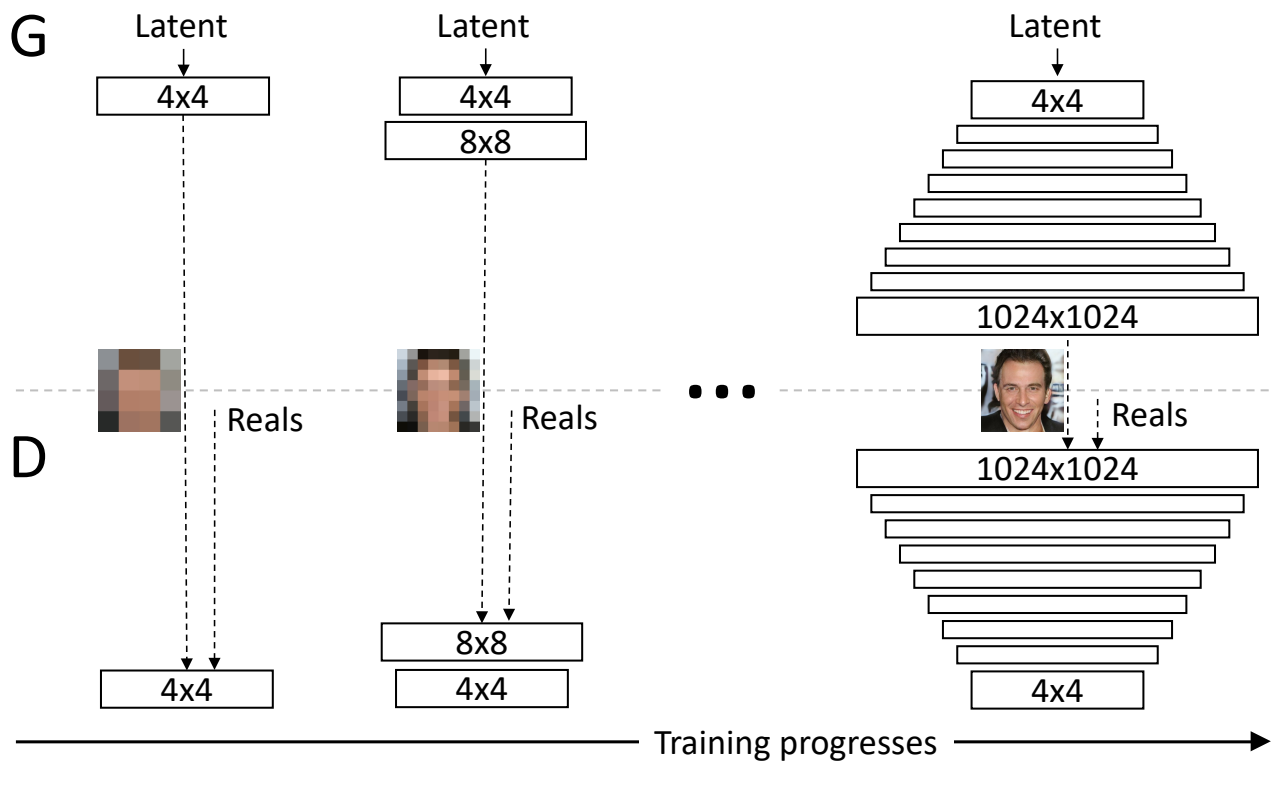
\includegraphics[width=\textwidth*4/5]{chapter1/proggan}
	\caption[Progressive growing of Generative Adversarial Networks]{Progressive growing of Generative Adversarial Networks. Convolutional layers are added throughout the learning process, each time doubling the dimension of the generated images.}
	\label{fig:proggan}
\end{figure}

This approach was extended  with tricks for mitigating its instability \citep{Salimans2016}, such as adding batch normalization \citep{Ioffe2015}, smoothing the 0/1 label used for training the discriminator or adding noise to the discriminator's input \citep{Sonderby2017}. They effectively helped stabilizing the training process. However, the \ac{DCGAN} approach remains limited in both the visual quality of the generated samples and in its ability to generate high-dimension images.

\textbf{Progressive GAN} \citep{Karras2017} first enabled high-dimensional image generation with GANs by progressively adding convolutional layers in the generator and the discriminator during training. Thus, the training starts with low-dimension images and progressively increase the dimension of the images throughout the learning process, which is illustrated in Figure \ref{fig:proggan}. This approach yielded the first high-quality, high-definition images generated with \ac{GANs}.

\begin{figure}
	\centering
	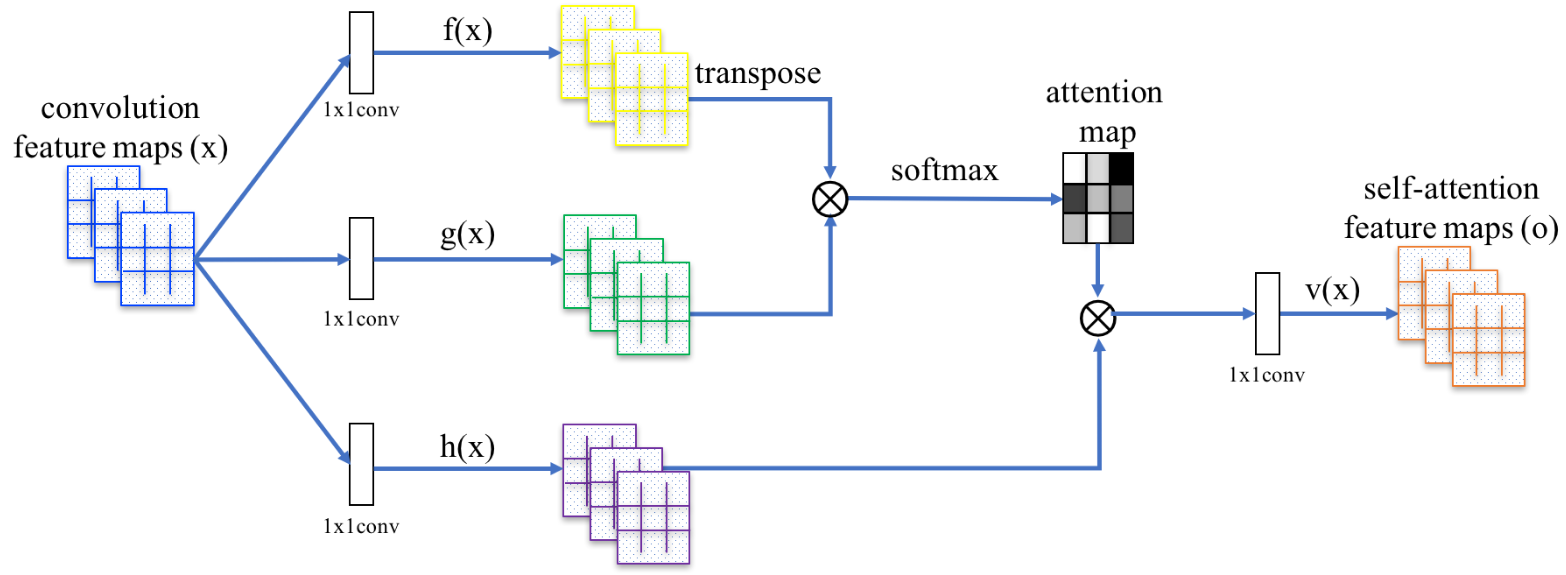
\includegraphics[width=\textwidth]{chapter1/sagan}
	\caption[Self-attention module]{Self-attention module for the SAGAN approach. The $\bigotimes$ denotes matrix multiplication. Figure by \citet{Zhang2018}}
	\label{fig:sagan}
\end{figure}

\textbf{Self-Attention GAN (SAGAN)} \citep{Zhang2018} implements attention-driven  mechanisms in \ac{GANs} to model \textit{long-range dependencies}. In most of the previous approaches, such as LAPGAN, DCGAN or Progressive GAN, the images are successively upscaled using convolutional layers. This causes issues in high-dimension, as some parts of the generated image could be inconsistent with each other due to the spatially local nature of convolutions. Self-attention propose to use non-local modeling as a solution to this issue. In the SAGAN approach, this is done by computing self-attention feature maps (see Figure \ref{fig:sagan}) that are then added to the convolution feature maps. 

\subsection{Augmenting the objective}
\label{subs:augmented_objectives}

Another common design approach for both stabilizing the training process and increasing diversity among the generated samples is to extend the \ac{GAN} objective with additional conditioning costs.

Training a \ac{GAN} in a supervised way with conditioning approaches such as Conditional GAN \citep{Mirza2014}, Auxiliary Classifier GAN \citep{Odena2016} or TripleGAN \citep{Li2017} (see Section \ref{subs:CGAN}) can enhance both the visual quality as well as the diversity among the generated samples. Indeed, GANs seem to take profit from the supervision added by the use of labels during the training process, even though it requires labeled data.

Another category of approaches aim to include an inference process into the GAN framework to retrieve the input noise from a generated sample, that is obtaining a function $I$ such that $I(\G(\vz)) = \vz, \vz \in \p{Z}$. \textbf{Artificially Learned Inference (ALI)} \citep{Dumoulin2016} and \textbf{Bidirectional GAN (BiGAN)} \citep{Donahue2017} are two similar approaches that aim to train a neural network $I: \spaceX \rightarrow \spaceZ$ as an inference mechanism. By providing the discriminator with either the input noise $\vz$ or the input noise $I(\vx)$ inferred from the real sample $\vx$ (see Figure \ref{fig:ali}), the networks $G, D$ and the inference model $I$ are trained simultaneously by solving the problem
%
\begin{equation}
		\min_{\G,I}\max_\D \esp{\vx \sim \p{X}} \Big[\log(\D(\vx, I(\vx)))\Big] + \esp{\vz\sim\p{Z}} \Big[\log(1-\D(\G(\vz), \vz))\Big]
\end{equation}
%
The main interest of these approaches is that they increase the diversity among the generated samples, but the trained inference model serve several purposes.  For example, since the optimal generator and inference models $G^*$ and $I^*$ are inverse of each others, as $I^*(G^*(\vz)) = \vz, \vz\sim\p{Z}$ and $G^*(I^*(\vx)) = \vx, \vx\sim\p{X}$, this allow for approximating the likelihood of a sample using the \textit{change of variable formula} (see Equation \ref{eq:change_variable_formula}) by considering $I^* = G^{*^{-1}}$.

\begin{figure}[t]
	\centering
	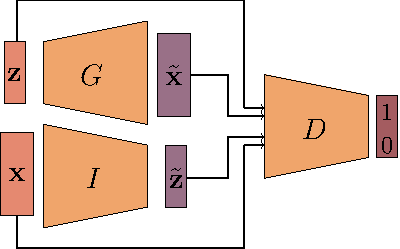
\includegraphics[width=\textwidth*3/5]{chapter1/ali}
	\caption[ALI/BiGAN approaches]{Artificially Learned Inference / Bidirectional GAN}
	\label{fig:ali}
\end{figure}

\textbf{Structured GAN} \citep{Deng2017} combines the supervised label-based conditioning with the inference-based approaches by adding both an inference model $I$ as well as a classifier $C$ that are trained jointly with the GAN. To do so, \citet{Deng2017} introduce two separate discriminators $\D_\vy$ and $\D_\vz$ that take respectively an image and its label, or an image and its corresponding noise in the latent space. The Structured GAN framework then consists in solving 
%
\begin{equation}
	\min_{\G,I,C}\max_D L_{\vx,\vy}(\G, \D, C) + L_{\vx, \vz}(\G, \D, I) + L_\vy(\G, \D, C) + L_\vz(\G, \D, I) \enspace,
\end{equation}
%
where $L_{\vx,\vy}$ and $L_{\vx, \vz}$ are adversarial losses, $L_\vy$ is a classification loss and $L_\vz$ is a disentanglement loss, that is a loss that aims to ensure that an inferred noise $I(\G(\vy, \vz)),  \vy\sim\p{Y}, \vz\sim\p{Z}$ is independent from the class label $\vy$. These losses takes the forms
%
\begin{align}
	L_{\vx, \vy} (\G, \D, C)&= \esp{\vx\sim\p{X}}\Big[\log\D_\vy(\vx, C(\vx))\Big] + \esp{\vy\sim\p{Y}\\\vz\sim\p{Z}} \Big[\log(\D_\vy(\G(\vy, \vz),  \vy))\Big]\\
	L_{\vx,\vz} (\G, \D, I)&= \esp{\vx\sim\p{X}}\Big[\log\D_\vz(\vx, I(\vx))\Big] + \esp{\vy\sim\p{Y}\\\vz\sim\p{Z}} \Big[\log(\D_\vz(\G(\vy, \vz),  \vz))\Big]\nonumber \\
	L_\vy(\G,\D, C)	&= - \esp{(\vx, \vy) \sim \p{X,Y}} \Big[\sum_{i=1}^{n}\vy_i C(\vx)_i\Big] - \esp{\vy \sim \p{Y} \\ \vz \sim \p{Z}} \Big[\sum_{i=1}^{n}\vy_i C(G(\vz))_i\Big] \nonumber \\
	L_\vz(\G, \D, I) &= - \esp{\vy_1, \vy_2\sim\p{Y}\\\vz \sim\p{Z}} \Big[||I(\G(\vy_1, \vz)) - I(\G(\vy_2, \vz)) ||^2_2\Big] \enspace.
\end{align}
%
Another method for conditioning GANs is \textbf{Packing GAN (PacGAN)} \citep{Lin2018}. This technique, designed to help with the diversity issues of GANs, consists in using sets of samples as input to the discriminator instead of single ones
%
\begin{equation}
	L_{PacGAN} = \esp{(\vx_1, ..., \vx_l) \sim \p{X}} \Big[\log(\D((\vx_1, ..., \vx_l)))\Big] + \esp{(\vz_1,...,\vz_l)} \Big[\log(1-\D((\G(\vz_1), ..., \G(\vz_l))))\Big] \enspace.
\end{equation}
%
 Since the real images $\vx_1, ..., \vx_l$ should always be different from each other, the task of the discriminator becomes very easy if the generator collapsed, that is if the generated samples $\G(\vz_1), ..., \G(\vz_l)$ are similar. This approach, albeit computationally more expensive than the classical \ac{GAN} framework because of the $l$ generated samples needed to train the discriminator, is very effective in preventing mode collapse.

Conversely to these conditioning approaches, several works showed that constraining the discriminator to be Lipschitz continuous \citep{Arjovsky2017a, Arjovsky2017, Qi2018} improved the stability of the training process. \textbf{Spectral Normalization} \citep{Miyato2018} show that normalizing the weights of the discriminator using the spectral norm of its weight matrix $\mw\in\spaceR^{n\times m}$, as 
%
\begin{equation}
	\mw' = \frac{\mw}{\sigma(\mw)}\enspace,
\end{equation}
%
with $\sigma(\mw)$ being the spectral norm\footnote{The spectral norm $\sigma(\mw)$ of a matrix $\mw$ is its maximum singular value} of $\mw$, is sufficient to ensure that the discriminator is 1-Lipschitz. Since computing the spectral norm for each training step is computationally expensive, the authors propose to use the \textit{power method} \citep{Golub2000} to compute a fast approximation of the spectral norm. This is done by sampling random vectors $\vu\in\spaceR^n$ and $\vv\in\spaceR^m$ and iteratively updating them as
%
\begin{equation}
	\vv \leftarrow \frac{\mw^\top\mw\vu}{||\mw^\top\mw\vu||_2},  \enspace \vu \leftarrow  \frac{\mw\vv}{||\mw\vv||_2} \enspace,
\end{equation}
%
then approximate the spectral norm as
%
\begin{equation}
	\sigma(\mw) \approx \vu^\top W\vv \enspace.
\end{equation}
%
This technique showed excellent results in stabilizing the GAN training process, notably allowing for learning a conditional generative model that was able to generate samples from the 1000 classes of the ImageNet dataset \citep{Deng2009}.

\section{A note on the  evaluation of  GANs}
\label{subs:evaluation_methods}

Unlike discriminative models, evaluating and comparing generative models is a non-trivial task. Two approaches can be envisioned: evaluating the \textit{intrinsic} quality of generated samples with ad-hoc criteria or directly evaluating the likelihood of the generated samples. However, unlike \ac{VAE}s and flow-based models, \ac{GAN}s offer no explicit way to evaluate or approximate the likelihood of the generated samples. Thus, a significant part of the \ac{GAN} literature resorts to a subjective visual evaluation of the generated samples. 

In order to provide a more precise evaluation of the visual quality of generated samples, two ad-hoc methods; the Inception Score (\ac{IS}) \citep{Salimans2016} and Fréchet Inception Distance (\ac{FID}) \citep{Heusel2017} were proposed, which both make use of a pre-trained Inception v3 model \citep{Szegedy2016}, a deep classifier trained on the ImageNet dataset \citep{Deng2009}.

\textbf{Inception Score (\ac{IS})}) \citep{Salimans2016} is based on the evaluation of the entropy of the labels $\vy$ predicted by the Inception classifier of generated data. High-fidelity samples should be easier to classify and therefore have a conditional label distribution $\pg{Y|X}$ with low entropy. In addition to the high quality, the samples should be diverse, therefore the marginal distribution 
%
\begin{equation}
	\pg{Y} = \int_{\setZ}\pg{Y|X=\G(\vz)}d\vz
\end{equation}
%
should have a high entropy. By combining these two requirements, the \ac{IS} is formulated as 
%
\begin{equation}
	\text{IS}(\vy) = \exp\Big[\esp{\vx\sim\pg{X}} \DKL{\pg{Y | X}}{\pg{Y}}\Big] \enspace .
\end{equation}
%
Although it has been widely used, \ac{IS} has shown major issues \citep{Barratt2018} that raise from the use of the conditional label distribution. Most notably, examples that are correctly classified are not necessarily of the highest quality and the pre-determined label classes can skew the estimation of the marginal distribution $p_\G(\vy)$.

The \textbf{Fréchet Inception Distance (\ac{FID})} \citep{Heusel2017}  differs from \ac{IS} since it evaluates a distance between the distributions of visual features computed on real and generated data, instead of relying on the labels. These features are extracted at the penultimate layer of the Inception classifier. The distributions of these features are assumed Gaussian, so that the Fréchet distance (or Wasserstein-2 distance) can be computed as
%
\begin{equation}
	FID = ||\mu – \mu_\G||^2 + Tr(\Sigma + \Sigma_\G – 2\sqrt{\Sigma\times\Sigma_\G}) \enspace ,
\end{equation}
%
where $\mathcal{N}(\mu, \Sigma)$ and $\mathcal{N}(\mu_\G, \Sigma_\G)$ are the distributions of the extracted features of the real and generated data, respectively. \ac{FID} is considered more robust than 
\ac{IS} \citep{Barratt2018} and has been either completing or replacing the use of \ac{IS} in recent works.

However, while these two metrics are considered to be the gold standard for evaluating \ac{GAN}s, their reliance on the pre-trained Inception model may be an issue. Indeed, they behave well when used to compare models learned on natural images datasets such as ImageNet, but they cannot directly extend to other datasets such as medical images or 3D images. A solution to consider is the training of another classifier network on a more adapted dataset, provided labeled data is available.

For the sake of completeness, we can also refer to some other notable (albeit less commonly used) metrics for evaluating visual quality  \citep{Borji2018}: the \textbf{Parzen window} (or kernel density) estimation \citep{Parzen1962} aim to estimate the likelihood of the generated samples; the \textbf{Sliced Wasserstein Distance} \citep{Julien2011} is an efficient approximation of the Earth-Mover (or Wasserstein) distance; the  \textbf{Kernel Inception Distance} \citep{Binkowski2018} is a recent metric that evaluates the maximum mean discrepancy between Inception features with a polynomial kernel.

Finally it is to note that for conditioned models, computing the aforementioned metrics does not inform on the quality of the conditioning. However, since the conditioning usually requires either labels or prior information, they can usually be used to evaluate conditioned models, for example predicting the labels of generated samples with a pre-trained classifier and computing the error between the predicted label and the original one.

\begin{figure}
	\centering
	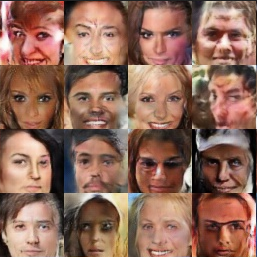
\includegraphics[width=\textwidth*3/10]{chapter1/dcgan_samples}	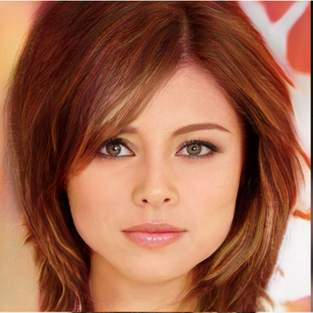
\includegraphics[width=\textwidth*3/10]{chapter1/proggan_sample}	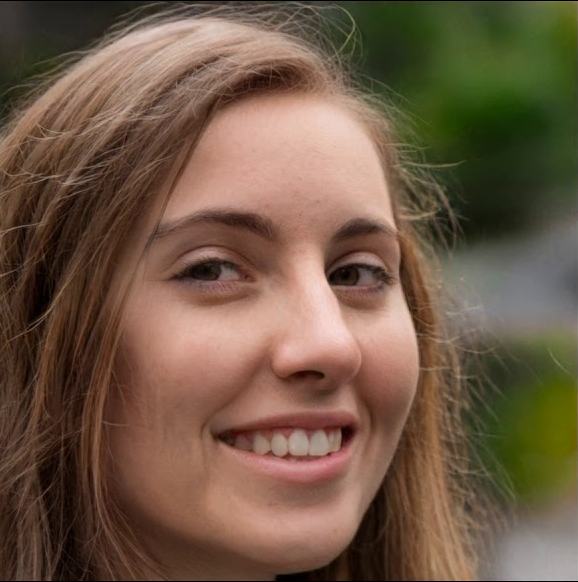
\includegraphics[width=\textwidth*3/10]{chapter1/stylegan2_sample}
	\caption[Evolution of the visual quality of generated images]{Evolution of the visual quality of generated images from 2014 to 2020, using the CelebA(-HQ) \citep{Liu2015} datasets. Left: DCGAN \citep{Radford2015}, Center: ProgGAN \citep{Karras2017}, Right: StyleGAN2 \citep{Karras2020}}
\end{figure}

\section{Conclusion}

In this chapter, we introduce the Generative Adversarial Network (\ac{GANs}) framework, which consists in a pair of neural networks, namely the generator and discriminator, that conjointly learn to model a complex data distribution by minimizing a divergence between the real data distribution and this modeled one. We present some of the techniques for conditioning modeling with GANs, from simply providing the GAN models with labels to adding a supervised auxiliary task to the training process. We present domain-transfer approaches with GANs, that is transferring an image from a data domain to another (for example images of infra-red to color images), most notably the cycle-consistent approaches that do not rely on hard-to-obtain paired data. 

We expose some of the limitations of the GAN framework, most notably the stability issues of the training process, the lack of diversity among the generated samples and the difficulty to produce high-quality, high-dimension images.  We review recent research works that aim to solve these issues, among them variants of the loss functions, changes to the architectures and advanced conditioning techniques. We also expose the difficulties of evaluating generative models and present common solutions for assessing the visual quality of generated samples.






